\chapter{Estrategia de modelos en entornos virtualizados}

Con el fin de abordar de manera ordenada la complejidad del sistema y validar progresivamente cada uno de sus componentes, se adoptó una estrategia basada en la construcción de modelos incrementales. Estos modelos permiten simular, probar y verificar distintas funcionalidades antes de integrarlas en la solución final.

Los modelos descritos a continuación tienen como finalidad:
\begin{itemize}
    \item Ligar problemas concretos a cada modelo y resolverlos de forma independiente. % Tener que debuggear todos en un solo modelo puede ser muy complejo.
    \item Obtener una solución funcional en un entorno virtualizado como último paso previo a probarla sobre \textit{hardware} real.
\end{itemize}

% Explicar la estructura del capítulo:
% - Que se valida
% - Que queda fuera del alcance
% - Descripción
% - Diagrama esquema físico
% - Explicación de cada componente
% - en cada modelo describir lo que se usa de cada tecnología, explicación en detalle




\section{Sistema mínimo}

Se propuso un primer modelo de baja complejidad complementario a la lectura de la documentación de WireGuard. La finalidad de este es familiarizarse con la configuración de un túnel VPN y su funcionamiento a través del análisis de paquetes de red. En el esquema de la figura \ref{diag:wg_minimal} se representa la topología de este ensayo, implementada sobre GNS3.

\begin{figure}[h!]
    \centering
    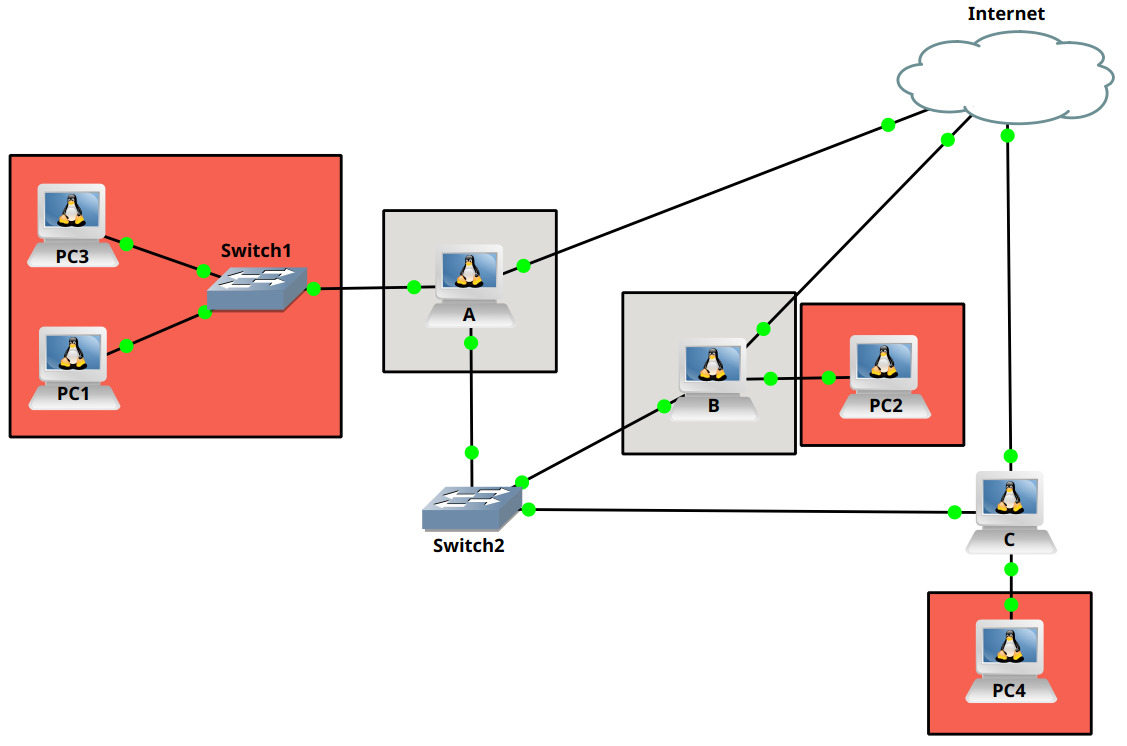
\includegraphics[width=0.6\textwidth]{../images/gns3_1.png}
    \caption{Otro esquema mejorcito.}
    \label{diag:wg_minimal}
\end{figure}

En una siguiente iteración de este modelo se descartó la utilización de GNS3 y se optó por instanciar cada VM en QEMU, y de esta manera adquirir mayor control sobre los dispositivos de red emulados. Un ejemplo de esto es la posibilidad de observar los parámetros PCI de las interfaces de red, lo cual es relevante para la implementación del \textit{passthrough} de las mismas en la solución final. 

Sobre este modelo además puede validarse el correcto funcionamiento de un kernel Linux modificado que luego se utilizará en cada VMM de seL4.

\section{Sistema completo usando máquinas virtuales}
Una vez planteada la arquitectura lógica del sistema, se procede a su simulación en GNS3. Este modelo permite limitar la complejidad de implementar la arquitectura a configurar la interconexión de las VMs que conforman el encriptador.

Este modelo tiene como objetivo validar la arquitectura lógica propuesta y verificar las funcionalidades de red pretendidas para el encriptador como puede ser el \textit{split-tunneling}.

En la figura \ref{diag:gns3_2} se muestra la topología de red utilizada en GNS3 para simular el sistema completo. El encriptador se implementa como la interconexión mediante interfaces de red de tres VMs independientes.

\begin{figure}[h!]
    \centering
    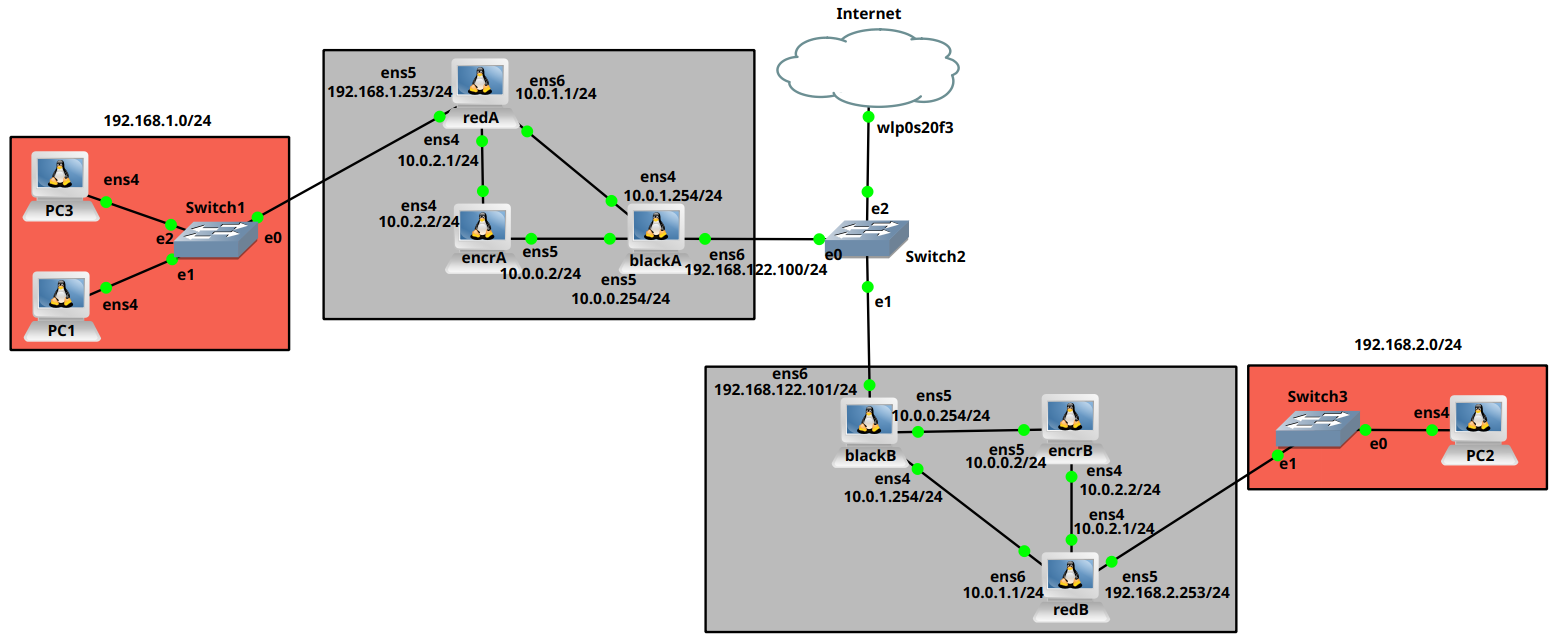
\includegraphics[width=0.8\textwidth]{../images/gns3_2.png}
    \caption{Otro esquema mejorcito.}
    \label{diag:gns3_2}
\end{figure}

Como \textit{output} de este modelo se obtienen las configuraciones de red necesarias (tablas de enrutamiento, reglas de firewall, etc.) para darle funcionalidad al encriptador. Estas configuraciones se utilizarán posteriormente en la solución.

% \section{Sistema mínimo con kernel Linux modificado}

% En una siguiente iteración 

% \begin{itemize}
%     \item Se utiliza QEMU para emular un sistema con un kernel Linux modificado que soporta WireGuard.
%     \item Dos instancias de QEMU.
%     \item Captura de Wireshark.
% \end{itemize}

\section{Sistema completo sobre seL4}
\begin{itemize}
    \item 4 instancias de QEMU: 2 PCs y 2 encriptadores.
    \item Descripción de zmq\_samples. Virtual Switch. ZeroMQ. Esquemas. 
\end{itemize}

\noindent\rule{\textwidth}{0.4pt}
%%%%%%%%%%%%%%%%%%%%%%%%%%%%%%%%%%%%%%%%%%%%%%%%%%%%%%%%%%%%%%





\section{Resumen}
Tabla: modelo, nivel de complejidad, validaciones
